\documentclass[article,11pt,onecolumn,final]{IEEEtran}
\usepackage{epsfig,latexsym,amsfonts,amsmath,amssymb,verbatim,cite,mathrsfs}
\usepackage{graphicx}
\usepackage{float}
\usepackage[dvips]{color}

\newtheorem{theorem}{Theorem}

\title{Passive Bistatic Radar using WiFi for Indoor Localization}

\author{\IEEEauthorblockN{Alexander Tooke and Ernest Carozza}  \\
\IEEEauthorblockA{Department of Electrical and Computer Engineering\\ 
Boston University
}}

\begin{document}

\maketitle
\begin{abstract}
As wireless networks have become commonplace in homes and offices, the opportunity arises to use
these signals for localization of a person or other target. Applications could range from improving indoor
location in the absence of GPS signals to locating an intruder inside a building. This project will explore
applying bistatic radar techniques to indoor localization of a target in an environment with IEEE 802.11
transmissions. This study surveys the feasibility of passive bistatic radar
using WiFi under ray tracing simulations of indoor fading. Using these simulations, bistatic radar techniques are
implemented to detect moving targets. This study finds that in low noise scenarios with few walls, the
techniques are successfully able to detect a moving target. The simulation approach in this paper 
provides an inexpensive platform for studying passive bistatic radar using WiFi and how the properties of
the environment can impact the effectiveness of these techniques.
\end{abstract}

\section{Introduction and motivation} 
Passive radar is a field that has relatively recently gained interest and traction due to the abundance of
RF emissions for communication purposes, covert and inexpensive receivers, and the rise of powerful
computers for implementing sophisticated signal processing algorithms. "WiFi radar" is an even newer
field that aims to use 802.11 emissions from standard noncooperative routers to perform indoor
localization. There are many potential applications of this technology: use as a supplement to GPS,
which typically has too low of a signal strength indoors to adequately track, track equipment in a
warehouse or factory, or detect targets using standard, everyday equipment without their knowledge as
a part of a security, surveillance or search and rescue system.

There already exist well known radar detection and tracking algorithms in the bistatic case, where the
transmitter and receiver are not collocated. However, standard radar systems have complete freedom
over their transmitted waveform and can therefore optimize for target tracking performance. One major
challenge in passive radar systems is the fact that the system has no control over the waveform, which
typically is a communication system waveform that is less than ideal for target localization. WiFi radar
poses the additional challenge that the multipath environment is extremely dense indoors, but has the
significant benefit that 802.11 devices are extremely widespread and commonplace.

The basic, first level construct in typical modern radar systems is a range-Doppler map -- a 2D plot of
signal power as a function of time delay and received Doppler shift. From this, high power level spots in
this map can be inferred to be targets at a specific range and range-rate, and targets that repeatedly
appear in these maps over time can be tracked. This project aims to form range-Doppler maps from
simulated data using a variety of proposed algorithms.

\section{Problem Statement} 
Our goal is to first simulate a simple indoor scenario with both stationary and moving targets using 
pre-existing OFDM waveform simulations and ray tracing. Total received signal at the receive antenna is modeled as

\begin{align*}
 s(t) = \sum_{l=1}^L A_l u(t-\tau_l)e^{j 2 \pi f_l t} + \sum_{m=1}^M A_m u(t-\tau_m)e^{j 2\pi f_m t} +
        \sum_{n=1}^N A_n u(t-\tau_n)e^{j 2 \pi f_n t} + A_{Dir} u(t-\tau_{Dir})
\end{align*}

Where $u(t)$ is the transmitted signal, there are $L$ targets, each scaled by $A_l$ in amplitude and time
delayed by $\tau_l$. Similarly, there are $M$ multipath returns and $N$ clutter returns all scaled and time delayed similarly, and finally the direct path return, which arrives first. This is given in \cite{Chetty} and was discussed in class.

We will calculate the ambiguity function of the simulated data, given by

\begin{align*}
\big|\int_{-\infty}^{\infty} s(t)s^*(t-\tau)e^{-j2\pi f_d t}dt \big|
\end{align*}

Which essentially provides useful information about the suitability of the OFDM WiFi waveform as a
radar signal, such as range resolution and Doppler resolution. Finally, we will implement range-Doppler
map forming algorithms as described in \cite{Colone2012} and explain how these maps would be used to localize
targets.


\section{Main Results}

The general approach of a radar system is to transmit a known signal then test how well the received signal correlates with delay and Doppler shifted versions of the original signal. In this study, 1 second of 802.11g OFDM transmissions are used as the transmitted signal. The channel is estimated through a ray tracing simulation in an environment with walls and a moving target. The simulated OFDM transmissions are convolved with the channel impulse response and white Gaussian noise is added to yield the signal at the receiver. Finally, a 2D range-Doppler map is generated by correlating the received signal with delay and Doppler shifted versions of the transmitted signal. A visual inspection of these 2D plots provides insight into the position and movement of a target.

\subsection{Modeling the Channel}

To start, we implemented a ray tracing simulation that calculates the channel impulse response for each pulse time. The approach taken in this study follows that in \cite{Holt}. The goal is to model the impulse response

\begin{align*}
 h(t) = \sum_{k=0}^{n} \beta_k e^{-j \theta_k} p(t - \tau_k) 
\end{align*}

where for signal path $k$, $\beta_k$ is the gain, $\theta_k$ is the phase for a sinusoid with a certain frequency, and $\tau_k$ is the propagation time. This is difficult to model exactly, so instead a sampled, discrete impulse response $h_l[m]$ is estimated using this simulation. 

As an impulse is transmitted, the signal is transmitted in all directions with equal strength. This is modeled by a number of discrete rays with a corresponding cone width. At each time step in the simulation, each ray moves in its current direction, and its width increases. Calculation of intersection with walls is only performed on the center line segment of each ray, so a large number of rays may be needed to keep the simulation accurate. 

In implementation, it was found to be easier to model each ray as a triangle instead of a cone, and time step of a ray as a section of the triangle (a trapezoid) rather than as a section cone. This was due to the need to calculate intersections with walls and the receiver along with the fact that these calculations are easier with lines that with curves. The triangle representing each ray has one point at the transmitter and two points each $r(t)$ from the transmitter with an angle of $2 \pi/N_{rays}$ degrees between them. The size of the outside edge of the triangle, called the cone width $D_{cone}$ can be found using the law of cosines

\begin{align*}
D_{cone}(t)^2 &= r^2 + r^2 - 2(r)(r)cos(\frac{2 \pi}{N_{rays}}) \\
              &= 2r^2(1 - cos(\frac{2 \pi}{N_{rays}})) \\
D_{cone}(t) &= \sqrt{2r^2(1 - cos(\frac{2 \pi}{N_{rays}}))}
\end{align*}

To simplify the calculations, the environment is assumed to be two dimensional, and the effects of floors and ceilings are neglected. Walls are modeled as reflecting, transmitting, and absorbing some portion of the energy. The angles of transmission and reflection are function of the dialectric properties of the materials, but for simplicity the model in \cite{Holt} assumes the transmitted portion of a signal does not change direction, and the reflected portion of a signal travels at the angle corresponding to the angle of incidence with the wall. In both the cases of transmission and reflecting, the signal is attenuated. This study used the same model as \cite{Holt} where the gain of a ray decreases linearly with distance and is multiplied by a constant factor for traveling through walls.

\begin{align*}
 \beta_k = \frac{A}{r(t)} \prod_m a_{km} 
\end{align*}

where $A$ is the gain at a fixed distance from the transmitter, $r(t)$ is the distance traveled by the signal at time $t$, and $a_{km}$ is the gain coefficient for transmission or reflection from walls. Therefore, the simulation must keep track of the attenuation from walls for each ray. Additionally, when a signal reflects off a wall, its phase is shifted by $\pi$ radians. The simulation must also keep track of this phase difference, which will be discussed in more detail later.

At the beginning of a simulation, $N_{rays}$ rays are created at the transmitter. At each time step, the simulation calculates where each ray would advance to in this time period. It next checks whether the trapezoid over which each ray covers in this time step contains the receiver. If it does, the tap in the impulse response corresponding to the current time step is updated. In addition to the gain and time offset, the phase also needs to be captured. It is initially confusing to consider the phase of an impulse response, but for the moment we must consider the phase of a sinusoid at the carrier frequency arriving at time $t$. The impulse response for tap $l$ is set to 

\begin{align*}
\beta_{k} e^{-j \theta_k}
\end{align*}

where $\theta_k=\frac{2 \pi f_c \tau_k}{c} + l_k \pi$
and $l_k$ represents the number of wall reflections, accounting for the phase shift that occurs in this case. Keeping track of the phase is critical in order for Doppler shifted versions of the signal to correlate.

The selection of time step sizes (corresponding to sampling rate) determines the amount of time and range resolution. For example, if a sampling rate of 3GHz is used, each ray moves 0.1 meter per time step, so it is not possible to get better than 0.1 meter resolution. During development, high sampling rates were used to prove out the concepts. For example, in the scenario below, 3GHz sampling rate was used to generate the impulse response. In the first figure, the transmitter is in the left room, the target is in the right room, and the receiver is to the left of the two rooms. The target is moving at 1m/s to the right. The simulation is performed 4 times, each 0.25 seconds apart. Therefore, in the second plot, the target has moved 0.25 meters to the right, and so the signal has traveled 0.5 meter further than in the first. We see that the third nonzero tap, corresponding to the reflection off the target, moves 5 taps to the right in each plot. With a resolution of 0.1 meters per time step, this is exactly what we expect.

\begin{figure}[H]
\caption{Ray tracing the channel with a transmitter, receiver, target, and walls}
\centering
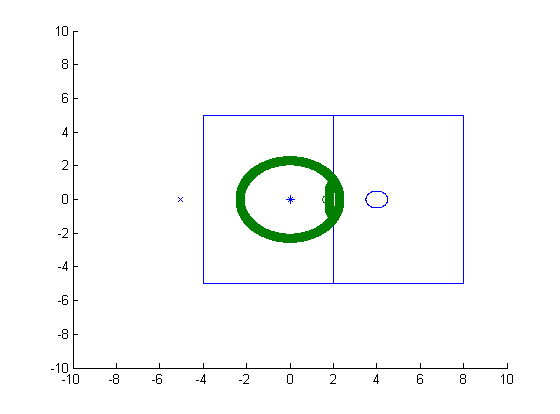
\includegraphics[width=400pt]{sim/simulation.png}  \\
\label{fig:Ray Tracing Channel}
\end{figure}

\begin{figure}[H]
\caption{$|h_l[m]|$ at m corresponding to t=[0, 0.25, 0.5, 0.75] seconds when sampling at 3GHz. Target moving 1 m/s to the right. }
\centering
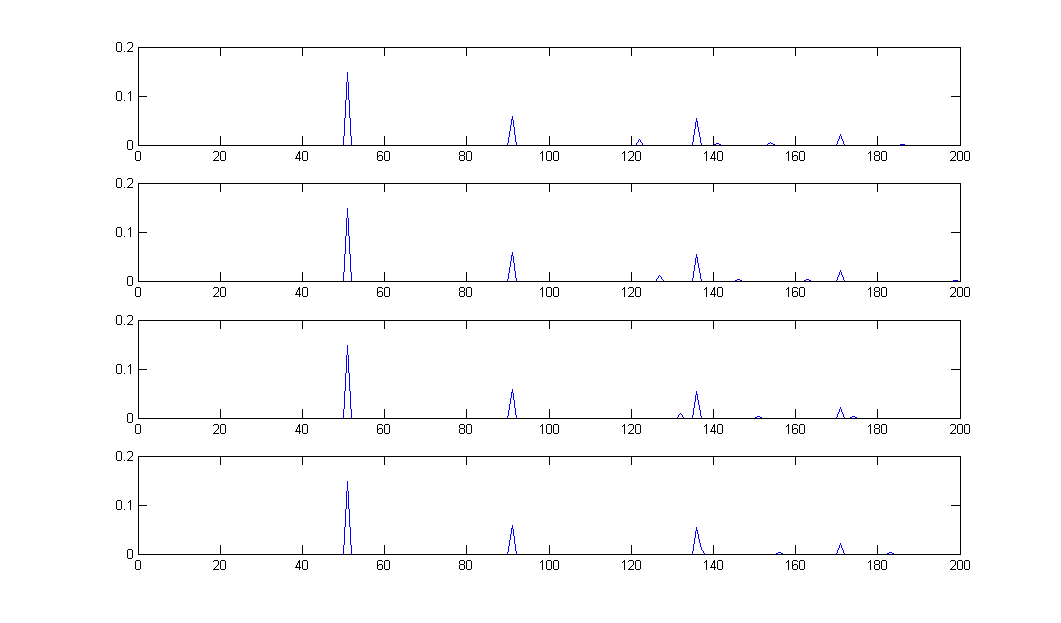
\includegraphics[width=400pt]{sim/impulse_response_taps.png}  
\label{fig:Impulse Response}
\end{figure}

For the purposes of using 802.11g transmissions, we are assuming that we are only capable of sampling at the rate of the bandwidth, 20Mhz. At this rate, each ray travels at $\frac{3*10^8}{20*10^6} = 15$ meters per time step, so this is the limit of resolution possible. We will elaborate on range and velocity resolution under the section on 802.11g waveform suitability for localization.

\subsection{Data Generation}
To perform the full simulation, the time varing channel impuse response is generated over the course of one second while sampling at 20MHz. To save computation time in simulation, $h_l$ is assumed to be constant for some period and is recomputed again. Experimentally, recomputing $h_l$ every $40 \mu s$, or 800 samples at 20 MHz yielded good results while speeding up computation by a factor of 800. Also, the number of time steps and corresponding taps was limited to save computation time. For example, if most of the information arrives in the first 5 time steps, the simulation may stop after 8 time steps. In this case, sampling $h_l[m]$ at 20Mhz for 1 second, using first 8 taps, holding constant for $4 \mu s$, results in a 25000x8 matrix for $h_l[m]$.

Next, we convolved simulated data obtained from a Simulink model available on the MATLAB file exchange \cite{Saxena} with the time varying channel impulse response to obtain an 802.11g OFDM waveform at varying data rates as it might propagate around a room with a moving target. This data was saved and run through an algorithm to calculate a range-Doppler map, which is a 2D range-velocity plot commonly used in radar. Additionally, the extensive cancellation-batches algorithm was used to clean up the raw complex samples input to the range-Doppler map forming algorithm.

\subsection{Range-Doppler Maps and Formation}

A range-Doppler map is the basis of most modern radar technology. A bistatic radar system measures range to a target by listening for both the "direct path" signal from the transmitter as well as the multipath echoes from targets in the environment, and then finding the time difference between these copies of the transmitted signal. In addition to simply finding the range, the system must discriminate these echoes by their Doppler shift, or implied velocity along the lines of sight between the transmitter to target and target to receiver. This discrimination by velocity enables the radar system to separate stationary items in the environment, such as ground, walls, and buildings which comprise the majority of return power, from targets of interest, which must be moving at some minimum velocity for the system to be effective.

Range Doppler maps are formed in a passive system as follows. It is essentially a matched filter in both range and velocity directions calculated by cross-correlating the aforementioned direct path signal $s_{ref}$ with the multipath echoes $s_{surv}$. Time indices that correlate well will have a large value of the cross correlation function in the range direction, which indicates the presence of a reflection at the distance corresponding to the time it takes light to propagate that distance. Frequency indices that correlate well with frequency shifted versions of the reference signal indicate the presence of Doppler shift, and targets at a given range and velocity should then show up as bright spots in the 2D cross-correlation map.

The 2D cross-correlation is given by

\begin{equation}
 C[l, p] = | \sum\limits_{i=0}^{N_{int}-1} s_{surv}[i]*s_{ref}^{*}[i - l]*e^{-j2\pi pi/N_{int}}|^2 
\end{equation}

where $l$ is the time delay bin which specifies range of echoes from that cell, $p$ is the Doppler bin which specifies Doppler shift frequency of that cell. $N_{int}$ is total number of raw samples in $s_{surv}$. Time delay bin and Doppler bin can both be converted to real quantities (meters and meters/second) as follows. The difference between the direct path distance and target bistatic range (known as the differential bistatic range) is $\delta R[l] = c*l*T_s$, where $T_s$ is equal to $1/f_s$, the A/D sample frequency. The Doppler bin p represents a Doppler frequency shift of $f_D[p] = p/(N_{int}T_s)$, which is converted into a Doppler velocity of $\delta v[p] = \lambda f_D[p]$. The quantity $N_{int}T_s$ is the CPI, or coherent processing interval, which determines Doppler resolution of the system as well as SNR gain, and for WiFi radar in our application is on the order of 1 second. At 2.4GHz this gives a Doppler resolution of 0.125 m/s.

According to \cite{Colone2012}, the 2D cross-correlation can be approximated by

\begin{equation} \label{eq:2dccapprox}
 C[l, p] = |\sum\limits_{m=0}^{M-1}e^{-j2\pi pi_m/N_{int}}\chi^{(m)}[l]|^2 
\end{equation}

with $M$ number of pulses in this CPI, $i_m$ the time index of the irst sample of $m$th pulse, and $\chi^{(m)}[l]$ the $l$th sample of the cross-correlation function in the time (range) direction for the $m$th pulse. This time cross correlation is calculated with the MATLAB xcorr function, separating OFDM pulses out by start time index and correlating the observed and reference signals over identical indices. So we have a cross-correlation of each pulse with each observed vector at the receiver; these are trimmed such that the first time index corresponds to a range of 0 meters and the last time index corresponds to the length of an 802.11g OFDM pulse (4 microseconds, 1200 meters when multiplied by the propagation speed of light).

Next we choose our number of Doppler bins by the maximum velocity we wish to detect. We used 128 for this simulation, which gives a maximum absolute value of velocity of 8 m/s, again assuming integration time of 1s. Shorter integration times yield less fine velocity grading but higher max/min detectable velocity while keeping number of bins constant. The correlation in the velocity direction is computed explicitly in our code as written in the above approximation.

\subsection{Suitability of 802.11g-spec OFDM Waveforms for Localization}
Radar range resolution in the best case can be estimated from the autocorrelation function of the transmitted pulse. A pulse reflected by a point scatterer will be heard by the receiver and correlated with the reference pulse as described above. In a conventional radar system, the ideal pulse would be an impulse; the cross correlation of the reference impulse and received echo would again be an impulse and the range resolution is infinite or extremely fine. In practice, an often used pulse is a linear frequency modulated (LFM) chirp over some bandwidth, since the 3dB width of the autocorrelation function over time of the LFM chirp is inversely proportional to its bandwidth -- roughly $\delta R = c / BW$ \cite{RadarBook}, and it is possible to send an appreciable amount when spreading the pulse over time. An additional important quantity is the peak-to-sidelobe ratio (PSR), since if the ratio is high, a single target could produce multiple returns with its real return at the peak and later returns at peak-PSR.

One difficulty in using OFDM waveforms for localization is their relatively poor autocorrelation properties, as shown by figure~\ref{fig:autocorr}. This was taken over the entire 1 second of simulated data we used and shows a PSR of around 14$dB$ over the first two delay taps. This will have the effect of spreading the target out over 5 delay bins (75 $m$) with a peak in the middle approximately 14dB higher before noise contributions. If this peak can be identified then the range resolution is 15 $m$, as estimated by the bandwidth criterion given above. 

\begin{figure}
	\caption{Autocorrelation function of 1 second of simulated WiFi data.}
	\centering
	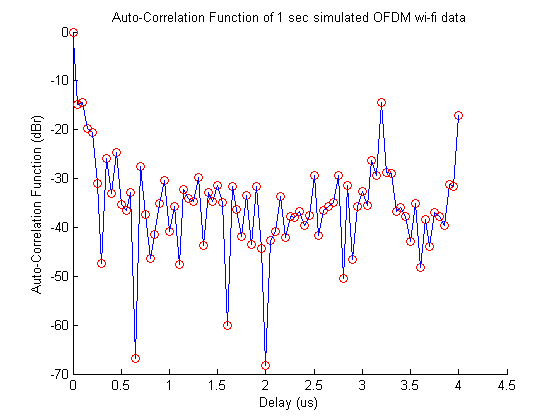
\includegraphics[width=400pt]{figures/autocorr.png}
	\label{fig:autocorr}
\end{figure}

Additionally, there is a range ambiguity that appears at 3.2 $\mu s$, corresponding to insertion of the 0.8 $\mu s$ guard interval in 802.11g OFDM pulses. This peak is approximately 13 $dB$ down, agreeing well with \cite{Colone2012}. This would present a significant problem; however, as shown in this paper, there exist reliable methods of correcting the pulse using windowing techniques. These techniques were not explored in this project, so the effect of the extra peak will be seen in our range-Doppler maps as a bright spot downrange.

Velocity or Doppler resolution is limited mainly by the integration time and has very nice autocorrelation properties over frequency, as shown in figure~\ref{fig:autocorrdopp}. This was generated using an integration time of 1 second, which is the integration time used throughout this paper including the simulation results and corresponds to a velocity resolution of 0.125 $m/s$ per bin, as mentioned above.

\begin{figure}[H]
	\caption{Autocorrelation function of WiFi data over Doppler shift dimension.}
	\centering
	\includegraphics[width=400pt]{figures/autocorrdopp.png}
	\label{fig:autocorrdopp}
\end{figure}

\section{Simulations}
\subsection{Simulating Indoor Channel with Multipath Fading}
The first step to simulate passive radar in an indoor setting is build a model for indoor fading. It is difficult to create a model that perfectly models walls, ceilings, furniture, etc. This project used an approach similar to that described in \cite{Holt}. This project implemented a ray tracing simulation to estimate the impulse response of the channel in an environment with walls and a moving object. 

\subsection{Choosing Scenarios}
Next, it is necessary to choose some representative scenarios. The first is simply a transmitter, receiver and target on a line with the target moving either toward or away from the receiver, as represented in figure ~\ref{fig:sim1}. We used both directions to ensure that the Doppler shift of the target was appearing at the correct location.

The final case is a more realistic scenario with the target and transmitter in a room and the receiver listening from outside. This is expected to more reasonably represent some of the difficulties in such an application, such as multipath from reflections off of walls and reduced received power level due to attenuation. This scenario is shown in ~\ref{fig:sim2}.

\subsection{Generating Range-Doppler Maps}
Finally, range-Doppler maps were generated using equation \eqref{eq:2dccapprox}. We will explain how these maps correspond to the simulation scenarios.

\subsection{Scenario 1 and 2 Results}

\begin{figure}[H]
	\caption{Graphical representation of first simulation scenario.}
	\centering
	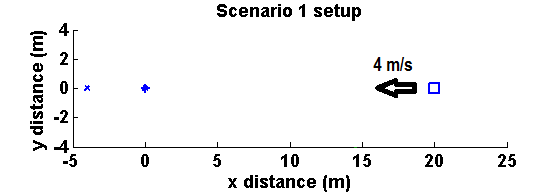
\includegraphics[width=400pt]{figures/sim1.png}
	\label{fig:sim1}
\end{figure}

\begin{figure}[H]
	\caption{Graphical representation of second simulation scenario.}
	\centering
	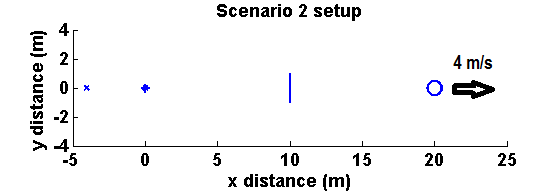
\includegraphics[width=400pt]{figures/sim2.png}
	\label{fig:sim2}
\end{figure}

\begin{figure}[H]
	\caption{Range-Doppler map of first simulation scenario}
	\centering
	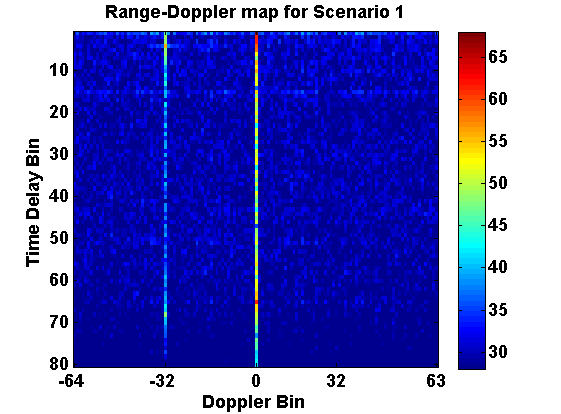
\includegraphics[width=400pt]{figures/rdm1.png}
	\label{fig:rdm1}
\end{figure}

\begin{figure}[H]
	\caption{Range-Doppler map of first simulation scenario}
	\centering
	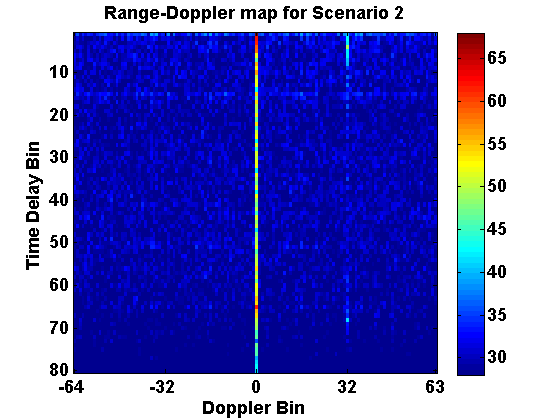
\includegraphics[width=400pt]{figures/rdm2.png}
	\label{fig:rdm2}
\end{figure}

The first scenario as seen in figures ~\ref{fig:sim1} and ~\ref{fig:rdm1} simply has the transmitter, receiver and target in a line with the target moving 4 $m/s$ toward the receiver and transmitter. There are no walls or added noise so we expect a strong return from the target to appear in time delay bin 4 and Doppler bin -32. Time bin 4 is 3 after the direct signal and corresponds to a two-way distance of 45m, Doppler bin -32 with bin spacing of 0.125 $m/s$ corresponds to the velocity of -4 $m/s$. Also note that both the direct path and target return spreads throughout all ranges due to the autocorrelation function issues pointed out earlier in the report. In fact, the 0 Doppler slice is exactly equal to the autocorrelation function of the data in this case. The range ambiguity at the 3.2 $\mu s$ time delay is also apparent and may be confused for additional targets by a full system.

The second scenario as seen in figures ~\ref{fig:sim2} and ~\ref{fig:rdm2} has the target moving in the opposite direction and additionally has a vertical wall placed in between the transmitter/receiver and target. All distances remain the same and the target return is seen on the other side of the RDM. Additionally, it is significantly reduced in power due to attenuation from the wall.

\subsection{Scenario 3 Results}

\begin{figure}[H]
	\caption{Graphical representation of third simulation scenario.}
	\centering
	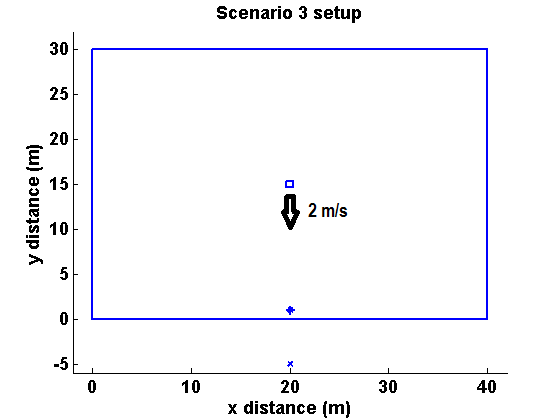
\includegraphics[width=400pt]{figures/sim3.png}
	\label{fig:sim3}
\end{figure}

\begin{figure}[H]
	\caption{Range-Doppler map of third simulation scenario}
	\centering
	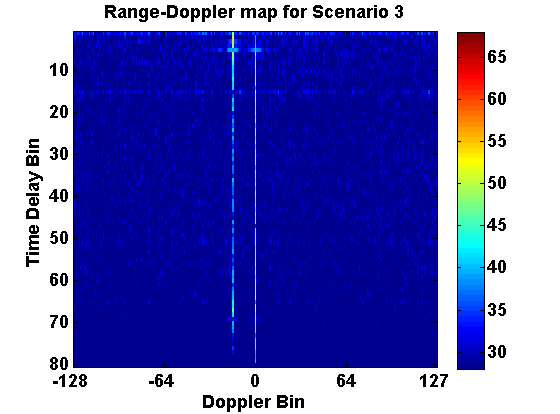
\includegraphics[width=400pt]{figures/rdm3.png}
	\label{fig:rdm3}
\end{figure}

\begin{figure}[H]
	\caption{Range-Doppler map of third simulation scenario zoomed in}
	\centering
	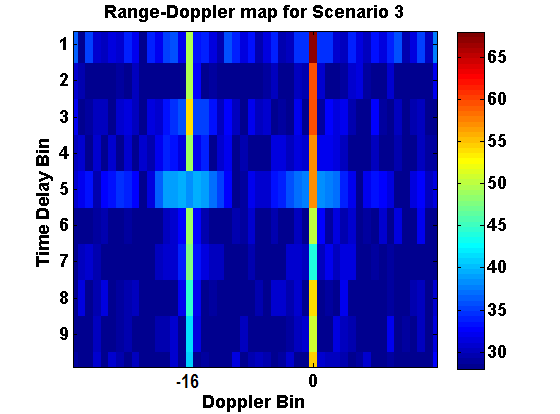
\includegraphics[width=400pt]{figures/rdm3zoom.png}
	\label{fig:rdm3zoom}
\end{figure}

This scenario has the transmitter and target inside a 40x30 $m^2$ room with its left corner at $[0, 0]$, the transmitter positioned at $[20, 1]$, the target positioned at $[20, 15]$ and moving at $-2 m/s$ in the $y$-direction, and the receiver positioned outside the room at $[20, -5]$. The expected two-way range in this case would be approximately 34 $m$ and would shrink to 30 $m$ after 1 second. Given our velocity spacing per bin, we expect the target to appear in Doppler bin -16 ($-2 / 0.125$). Given the 30 $m$ range, this means the target should appear 2 time delay bins following the direct path signal. Additionally, given the multipath environment, we see a weaker, Doppler-spread echo off of the back wall of the room, which has a 2-way range of an additional 30 $m$ and correspondingly appears 2 time bins later than the first echo.

\section{Concluding Remarks}
This study has shown the feasibility of detecting the position and movement of a indoor target using bistatic
radar techniques. The approach consisted of modeling the indoor channel using ray tracing, being sure to 
model changes in propagation time and phase due to a target moving. After convolving a simulated 802.11g
OFDM signal with the simulated time varing impulse response, the received signal is generated. The received
signal is correlated with delay and Doppler shifted versions of the original signal, and combinations that correlate
strongly indicate the range and speed of an object. In single, low noise scenarios the methodology has shown
to be sound and could lead to a practical solution.

Previous studies into passive bistatic radar have focused on real systems with measured data and expensive
acquisition systems. This study adds value in that by simulating the channel with some basic assumptions, there 
is a rapid and inexpensive way to study the same concepts. Furthermore, parameters such as reflectivity of
walls can be varied and the impact can be studied. This could be particularly useful for those who want to know
how to prevent others from performing this kind of analysis on their property.

There are some limitations in this study, for example that the ray tracing makes some simplifying assumptions, 
such as that floors and ceilings are neglected. The target in the ray tracing simulation is modeled as a 2D polyhedron, when it should probably just absorb a ray and proportionally reradiate over some angle. This is the reason that the target, receiver and transmitter were always in a line in our results: we were unsure whether the rays would ever bounce back to the receiver given how the ray tracing was implemented, generating the channel response takes a significant amount of time, and we ran into time constraints with the project due date. Reradiating would solve this issue but our simulation gets the idea across anyway. 

There is also some further work in academia with respect to bistatic
radar that could improve results, including how to reduce the inteference from very strong direct signal. One such algorithm, the Extensive Cancellation Algorithm - Batches (ECA-B) as presented in \cite{Colone2006}, \cite{Colone2009}, and \cite{Colone2012} was implemented as part of this project but did not work as expected and so was left out.In addition, with multiple receivers
in separate locations, it is possible that trilateration, as is used in GPS, could be used to fully localize a target in 2D or 3D space rather than in just range. This analysis would be necessary to build a complete localization solution.

A major simplifying assumption in this work is the lack of white Gaussian noise in the received signal, an effect we intended to model but left out due to time constraints. The effect of noise would basically be making the target more difficult to distinguish in the range-Doppler maps; instead of being 30 $dB$ above the typical noise floor it might be 10 $dB$ or even less, making it difficult or impossible to detect reliably. 

\begin{thebibliography}{100}

\bibitem{Chetty} Chetty, K.; Smith, G.E.; Woodbridge, K., "Through-the-Wall Sensing of Personnel Using Passive
Bistatic WiFi Radar at Standoff Distances," Geoscience and Remote Sensing, IEEE Transactions on ,
vol.50, no.4, pp.1218,1226, April 2012
doi: 10.1109/TGRS.2011.2164411

\bibitem{Maechler} Maechler, P.; Felber, N.; Kaeslin, H., "Compressive sensing for WiFi-based passive bistatic radar,"
Signal Processing Conference (EUSIPCO), 2012 Proceedings of the 20th European , vol., no.,
pp.1444,1448, 27-31 Aug. 2012

\bibitem{Buonanno} Buonanno, A.; D'Urso, M.; Palmieri, L., "Wifi-based passive bistatic radar by using moving target
indicator and least square adaptive filtering," Phased Array Systems \& Technology, 2013 IEEE
International Symposium on , vol., no., pp.174,179, 15-18 Oct. 2013

\bibitem{Colone2012} Colone, F.; Falcone, P.; Bongioanni, C.; Lombardo, P., "WiFi-Based Passive Bistatic Radar: Data
Processing Schemes and Experimental Results," Aerospace and Electronic Systems, IEEE Transactions
onAerospace and Electronic Signals, Vol. 48, no.2, pp.1061-1079, Apr. 2012

\bibitem{Hemple} Hemple, S., “Analysis and Simulation of Wireless ODFM Communications,” M.S. Thesis, Dept. of
Mathematics and Statistics, San Diego State Univ., San Diego, CA, Apr. 2012

\bibitem{Saxena} Saxena, A. (2012). "802.11g WLAN PHY Model," [Online]. Available: http://www.mathworks.com/matlabcentral/fileexchange/38073-802-11g-wlan-phy-model

\bibitem{Colone2011} Colone, F., “Ambiguity Function Analysis of Wireless LAN Transmissions for Passive Radar,”
Aerospace and Electronic Systems, IEEE Transactions on Aerospace and Electronic Systems, Vol. 47, No.1,
pp. 240-264, Jan. 2011

\bibitem{Holt} Holt, T.; Pahlavan, K.; Lee, J-F, "A graphical indoor radio channel simulator using 2D ray tracing," Personal, Indoor and Mobile Radio Communications, 1992. Proceedings, PIMRC '92., Third IEEE International Symposium on , vol., no., pp.411,416, 19-21 Oct 1992

\bibitem{Colone2009} Colone, F.; O'Hagan, D. W.; Lombardo, P.; Baker, C.J., "A Multistage Processing Algorithm for Disturbance Removal and Target Detection in Passive Bistatic Radar," IEEE Transactions on Aerospace and Electronic Systems, Vol. 45, no.2, Apr. 2009

\bibitem{Colone2006} Colone, F.; Cardinali, R.; Lombardo, P., "Cancellation of Clutter and Multipath in Passive Radar Using a Sequential Approach," IEEE Conference on Radar, Apr. 2006

\bibitem "IEEE Standard for Information Technology, Part 11: Wireless LAN Medium Access Control (MAC) and Physical Layer (PHY) specifications" IEEE Std 802.11-2012

\bibitem{RadarBook} M.A. Richards, J.A. Scheer, W.A. Holm, "Principles of Modern Radar: Basic Principles." Raleigh, NC: SciTech Publishing, 2010.


\end{thebibliography}

\end{document}
